% Created by tikzDevice version 0.10.1 on 2018-01-31 10:28:13
% !TEX encoding = UTF-8 Unicode
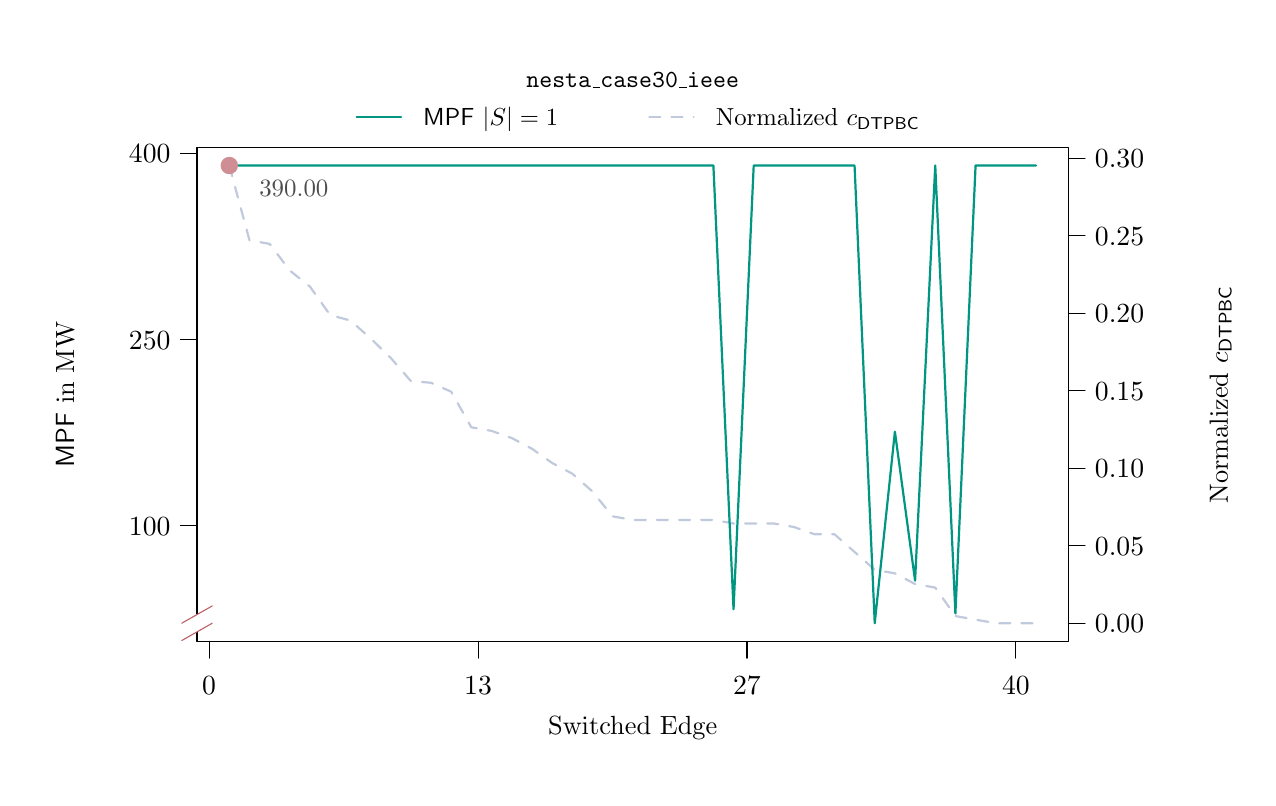
\begin{tikzpicture}[x=1pt,y=1pt]
\definecolor{fillColor}{RGB}{255,255,255}
\path[use as bounding box,fill=fillColor,fill opacity=0.00] (0,0) rectangle (440.85,271.01);
\begin{scope}
\path[clip] (  0.00,  0.00) rectangle (440.85,271.01);
\definecolor{drawColor}{RGB}{193,202,220}

\path[draw=drawColor,line width= 0.8pt,dash pattern=on 4pt off 4pt ,line join=round,line cap=round] ( 72.86,221.20) --
	( 80.15,194.17) --
	( 87.44,192.88) --
	( 94.73,183.23) --
	(102.01,177.44) --
	(109.30,167.14) --
	(116.59,165.21) --
	(123.88,158.78) --
	(131.17,151.70) --
	(138.45,143.33) --
	(145.74,142.69) --
	(153.03,139.47) --
	(160.32,126.60) --
	(167.61,125.31) --
	(174.89,122.74) --
	(182.18,118.88) --
	(189.47,113.73) --
	(196.76,109.87) --
	(204.05,103.44) --
	(211.34, 94.43) --
	(218.62, 93.14) --
	(225.91, 93.14) --
	(233.20, 93.14) --
	(240.49, 93.14) --
	(247.78, 93.14) --
	(255.06, 91.85) --
	(262.35, 91.85) --
	(269.64, 91.85) --
	(276.93, 90.56) --
	(284.22, 87.99) --
	(291.50, 87.99) --
	(298.79, 81.56) --
	(306.08, 75.12) --
	(313.37, 73.83) --
	(320.66, 69.97) --
	(327.95, 68.69) --
	(335.23, 58.39) --
	(342.52, 57.10) --
	(349.81, 55.82) --
	(357.10, 55.82) --
	(364.39, 55.82);
\end{scope}
\begin{scope}
\path[clip] (  0.00,  0.00) rectangle (440.85,271.01);
\definecolor{drawColor}{RGB}{0,0,0}

\path[draw=drawColor,line width= 0.4pt,line join=round,line cap=round] ( 61.20, 49.20) --
	(376.05, 49.20) --
	(376.05,227.81) --
	( 61.20,227.81) --
	( 61.20, 49.20);
\end{scope}
\begin{scope}
\path[clip] (  0.00,  0.00) rectangle (440.85,271.01);
\definecolor{drawColor}{RGB}{0,0,0}

\path[draw=drawColor,line width= 0.4pt,line join=round,line cap=round] (376.05, 55.82) -- (376.05,223.77);

\path[draw=drawColor,line width= 0.4pt,line join=round,line cap=round] (376.05, 55.82) -- (382.05, 55.82);

\path[draw=drawColor,line width= 0.4pt,line join=round,line cap=round] (376.05, 83.81) -- (382.05, 83.81);

\path[draw=drawColor,line width= 0.4pt,line join=round,line cap=round] (376.05,111.80) -- (382.05,111.80);

\path[draw=drawColor,line width= 0.4pt,line join=round,line cap=round] (376.05,139.79) -- (382.05,139.79);

\path[draw=drawColor,line width= 0.4pt,line join=round,line cap=round] (376.05,167.79) -- (382.05,167.79);

\path[draw=drawColor,line width= 0.4pt,line join=round,line cap=round] (376.05,195.78) -- (382.05,195.78);

\path[draw=drawColor,line width= 0.4pt,line join=round,line cap=round] (376.05,223.77) -- (382.05,223.77);

\node[text=drawColor,anchor=base west,inner sep=0pt, outer sep=0pt, scale=  1.00] at (385.65, 52.37) {0.00};

\node[text=drawColor,anchor=base west,inner sep=0pt, outer sep=0pt, scale=  1.00] at (385.65, 80.36) {0.05};

\node[text=drawColor,anchor=base west,inner sep=0pt, outer sep=0pt, scale=  1.00] at (385.65,108.36) {0.10};

\node[text=drawColor,anchor=base west,inner sep=0pt, outer sep=0pt, scale=  1.00] at (385.65,136.35) {0.15};

\node[text=drawColor,anchor=base west,inner sep=0pt, outer sep=0pt, scale=  1.00] at (385.65,164.34) {0.20};

\node[text=drawColor,anchor=base west,inner sep=0pt, outer sep=0pt, scale=  1.00] at (385.65,192.34) {0.25};

\node[text=drawColor,anchor=base west,inner sep=0pt, outer sep=0pt, scale=  1.00] at (385.65,220.33) {0.30};
\end{scope}
\begin{scope}
\path[clip] (  0.00,  0.00) rectangle (440.85,271.01);
\definecolor{drawColor}{RGB}{0,150,130}

\path[draw=drawColor,line width= 0.8pt,line join=round,line cap=round] (118.89,238.60) -- (134.91,238.60);
\definecolor{drawColor}{RGB}{193,202,220}

\path[draw=drawColor,line width= 0.8pt,dash pattern=on 4pt off 4pt ,line join=round,line cap=round] (224.63,238.60) -- (240.65,238.60);
\definecolor{drawColor}{RGB}{0,0,0}

\node[text=drawColor,anchor=base,inner sep=0pt, outer sep=0pt, scale=  0.89] at (218.62,249.28) {\texttt{nesta\_case30\_ieee}};

\node[text=drawColor,anchor=base west,inner sep=0pt, outer sep=0pt, scale=  0.89] at (142.92,235.54) {$\mathsf{MPF}~|S|=1$};

\node[text=drawColor,anchor=base west,inner sep=0pt, outer sep=0pt, scale=  0.89] at (248.66,235.54) {Normalized~$c_\mathsf{DTPBC}$};
\end{scope}
\begin{scope}
\path[clip] (  0.00,  0.00) rectangle (440.85,271.01);
\definecolor{drawColor}{RGB}{0,0,0}

\path[draw=drawColor,line width= 0.4pt,line join=round,line cap=round] ( 61.20, 90.98) -- ( 61.20,225.69);

\path[draw=drawColor,line width= 0.4pt,line join=round,line cap=round] ( 61.20, 90.98) -- ( 55.20, 90.98);

\path[draw=drawColor,line width= 0.4pt,line join=round,line cap=round] ( 61.20,158.33) -- ( 55.20,158.33);

\path[draw=drawColor,line width= 0.4pt,line join=round,line cap=round] ( 61.20,225.69) -- ( 55.20,225.69);

\node[text=drawColor,anchor=base east,inner sep=0pt, outer sep=0pt, scale=  1.00] at ( 51.60, 87.53) {100};

\node[text=drawColor,anchor=base east,inner sep=0pt, outer sep=0pt, scale=  1.00] at ( 51.60,154.89) {250};

\node[text=drawColor,anchor=base east,inner sep=0pt, outer sep=0pt, scale=  1.00] at ( 51.60,222.24) {400};
\end{scope}
\begin{scope}
\path[clip] (  0.00,  0.00) rectangle (440.85,271.01);
\definecolor{drawColor}{RGB}{255,255,255}
\definecolor{fillColor}{RGB}{255,255,255}

\path[draw=drawColor,line width= 0.4pt,line join=round,line cap=round,fill=fillColor] ( 55.69, 52.69) rectangle ( 66.71, 58.94);
\definecolor{drawColor}{RGB}{188,97,104}

\path[draw=drawColor,line width= 0.4pt,line join=round,line cap=round] ( 55.69, 49.56) -- ( 66.71, 55.82);

\path[draw=drawColor,line width= 0.4pt,line join=round,line cap=round] ( 55.69, 55.82) -- ( 66.71, 62.07);
\end{scope}
\begin{scope}
\path[clip] ( 61.20, 49.20) rectangle (376.05,227.81);
\definecolor{drawColor}{RGB}{0,150,130}

\path[draw=drawColor,line width= 0.8pt,line join=round,line cap=round] ( 72.86,221.20) --
	( 80.15,221.20) --
	( 87.44,221.20) --
	( 94.73,221.20) --
	(102.01,221.20) --
	(109.30,221.20) --
	(116.59,221.20) --
	(123.88,221.20) --
	(131.17,221.20) --
	(138.45,221.20) --
	(145.74,221.20) --
	(153.03,221.20) --
	(160.32,221.20) --
	(167.61,221.20) --
	(174.89,221.20) --
	(182.18,221.20) --
	(189.47,221.20) --
	(196.76,221.20) --
	(204.05,221.20) --
	(211.34,221.20) --
	(218.62,221.20) --
	(225.91,221.20) --
	(233.20,221.20) --
	(240.49,221.20) --
	(247.78,221.20) --
	(255.06, 60.87) --
	(262.35,221.20) --
	(269.64,221.20) --
	(276.93,221.20) --
	(284.22,221.20) --
	(291.50,221.20) --
	(298.79,221.20) --
	(306.08, 55.82) --
	(313.37,125.02) --
	(320.66, 71.19) --
	(327.95,221.20) --
	(335.23, 59.32) --
	(342.52,221.20) --
	(349.81,221.20) --
	(357.10,221.20) --
	(364.39,221.20);
\end{scope}
\begin{scope}
\path[clip] ( 61.20, 49.20) rectangle (376.05,227.81);
\definecolor{fillColor}{RGB}{207,142,147}

\path[fill=fillColor] ( 72.86,221.20) circle (  3.15);
\end{scope}
\begin{scope}
\path[clip] ( 61.20, 49.20) rectangle (376.05,227.81);
\definecolor{drawColor}{gray}{0.30}

\node[text=drawColor,anchor=base,inner sep=0pt, outer sep=0pt, scale=  0.90] at ( 96.18,210.04) {390.00};
\end{scope}
\begin{scope}
\path[clip] (  0.00,  0.00) rectangle (440.85,271.01);
\definecolor{drawColor}{RGB}{0,0,0}

\path[draw=drawColor,line width= 0.4pt,line join=round,line cap=round] ( 65.57, 49.20) -- (357.10, 49.20);

\path[draw=drawColor,line width= 0.4pt,line join=round,line cap=round] ( 65.57, 49.20) -- ( 65.57, 43.20);

\path[draw=drawColor,line width= 0.4pt,line join=round,line cap=round] (162.75, 49.20) -- (162.75, 43.20);

\path[draw=drawColor,line width= 0.4pt,line join=round,line cap=round] (259.92, 49.20) -- (259.92, 43.20);

\path[draw=drawColor,line width= 0.4pt,line join=round,line cap=round] (357.10, 49.20) -- (357.10, 43.20);

\node[text=drawColor,anchor=base,inner sep=0pt, outer sep=0pt, scale=  1.00] at ( 65.57, 30.00) {0};

\node[text=drawColor,anchor=base,inner sep=0pt, outer sep=0pt, scale=  1.00] at (162.75, 30.00) {13};

\node[text=drawColor,anchor=base,inner sep=0pt, outer sep=0pt, scale=  1.00] at (259.92, 30.00) {27};

\node[text=drawColor,anchor=base,inner sep=0pt, outer sep=0pt, scale=  1.00] at (357.10, 30.00) {40};

\node[text=drawColor,anchor=base,inner sep=0pt, outer sep=0pt, scale=  0.95] at (218.62, 15.60) {Switched Edge};

\node[text=drawColor,rotate= 90.00,anchor=base,inner sep=0pt, outer sep=0pt, scale=  0.95] at ( 16.80,138.51) {$\mathsf{MPF}$ in~$\mathrm{MW}$};

\node[text=drawColor,rotate= 90.00,anchor=base,inner sep=0pt, outer sep=0pt, scale=  0.95] at (433.65,138.51) {Normalized~$c_\mathsf{DTPBC}$};
\end{scope}
\end{tikzpicture}
